\documentclass[12pt,a4paper]{article}
\usepackage[utf8]{inputenc}
\usepackage{url}
\usepackage{hyperref}
\usepackage{float}
\usepackage[utf8]{inputenc}
\usepackage[english]{babel}
\usepackage{url}
\usepackage{graphicx, capt-of}
\usepackage{titletoc}
\usepackage{setspace}   %Allows double spacing with the \doublespacing command
\usepackage{authblk}
\usepackage{float}
\usepackage{geometry}
\usepackage{textcomp}

\usepackage{caption}
%\geometry{legalpaper, margin=1.2in}
\usepackage[usenames, dvipsnames]{color}
 
%Import the natbib package and sets a bibliography  and citation styles
\usepackage{natbib}
%Import siunitx packages so that tables can be centered
\usepackage{siunitx} 
\usepackage{multirow}
\sisetup{
  round-mode          = places, % Rounds numbers
  round-precision     = 2, % to 2 places
}
\usepackage{rotating}
\usepackage{subcaption}
\usepackage[table]{xcolor}

\newcounter{subfloat}
\renewcommand{\thesubfloat}{\alph{subfloat}}
\newcommand{\image}[2]{%
  \stepcounter{subfloat}%
  \begin{tabular}[t]{@{}c@{}}
  #2 \\
  \end{tabular}%
}

\definecolor{lightgray}{gray}{0.9}
\definecolor{lightblue}{rgb}{0.93,0.95,1.0}

\begin{document}
\pagenumbering{gobble}
{\fontfamily{phv}\selectfont}
\title{\Huge Exploring the Landscape of Glycan Structure\vspace{1cm}\\ \large  MSc Bioinformatics and Theoretical Systems Biology Project\vspace{11cm}}

\date{}

\author{\Large Steven Hargreaves\\
\normalsize CID 01453122 \\\vspace{0.5cm}
\normalsize Imperial College London \\
\normalsize Department of Life Sciences \\
\normalsize Word Count: 5479}


\maketitle
%\setcitestyle{numbers}
\newpage
\begin{abstract}
\pagenumbering{arabic}
\doublespacing
\noindent Glycans are highly prevalent in living organisms, and play keys roles in a variety of important biological processes such as cell signalling, immune reaction, viral infections and tumour cell proliferation. The difficulty of analysing glycan structures experimentally provides the motivation to develop reliable computational analysis techniques. A hindrance to this effort though is the complex tree-like structure of glycans, making them more difficult to analyse and compare than, for example, the linear chains of polypeptides in proteins. We describe a novel technique for measuring glycan similarity based upon a consideration of the biological reactions necessary for their synthesis, and which avoids the need to model tree structures. By analysing the similarities between 4111 glycans from a public database, we demonstrate that we can identify communities of glycans sharing the same or similar motifs, and that we can predict the presence of specific motifs in glycans which do not as yet have motif annotations.

% Include some numbers for Sternberg\\
% e.g. no. glycans (pre/post filtering steps), no. motifs, assortativity coeffs?\\

% The project report must include the word count on the title page (the number of words will be checked and failure to comply with the word limit will incur penalties)\\

% critically evaluated your results\\
% The Abstract
% should be structured (i.e. aims, methods, results, conclusion), be no more 
% than  one  side  of  paper  (in  written  reports).  Ideally  the  Abstract  should  cite  some  key numerical  results  rather  than  just  generalities.    Making  a  point  in  an  abstract  does  not remove  the  requirement  for  it  to  be  made  elsewhere  in  the  report.  The  report  must  be comprehensible even if the abstract is removed.  \\

\end{abstract}

\newpage
\begin{center}
\section*{Acknowledgements}
\doublespacing
Many thanks to John Pinney for his supervision and guidance during this project, and to Suhail Islam for technical assistance. The database and JSON file icons used in Figure \ref{fig:flowchart} were designed by Smashicons from Flaticon.
\end{center}
\newpage
\tableofcontents
\newpage
\section*{Abbreviations}
\doublespacing
\textit{GT:} Glycosyltransferase\\
\textit{JSON:} JavaScript Object Notation\\
\textit{RDF:} Resource Description Framework\\
\textit{SPARQL:} A recursive acronym for SPARQL Protocol and RDF Query Language\\
\textit{UPGMA:} Unweighted Pair Group Method with Arithmetic Mean\\
\textit{WURCS:} Web3 Unique Representation of Carbohydrate Structures\\
\textit{XML:} Extensible Markup Language\\
\addcontentsline{toc}{section}{Abbreviations} %adds it to the table of contents

\newpage
\section*{Glossary}
\addcontentsline{toc}{section}{Glossary}
\label{sec:glossary}
\doublespacing
\noindent{\textit{Anomericity:} The configuration, either axial ($\alpha$) or equatorial ($\beta$), of the OH-group at carbon number one of a monosaccharide.}\\\\
\noindent{\textit{Archeopteryx:} Phylogenetic tree visualisation software.}\\\\
\noindent{\textit{Binary adjacency matrix:} A square matrix in which elements represent the adjacency of pairs of vertices in a graph.}\\\\
\noindent{\textit{Glycan:} Compounds of monosaccharides linked glycosidically, which exist in free form or in covalent complexes with proteins or lipids .}\\\\
\noindent{\textit{Glycan motif:} A commonly occurring glycan substructure appearing in multiple glycans.}\\\\
\noindent{\textit{Glycosyltransferase:} An enzyme which catalyses glycosidic linkages.}\\\\
\noindent{\textit{GlyTouCan:} Online database of glycan structures.}\\\\
\noindent{\textit{Jaccard similarity coefficient:} A statistic for comparing the similarity of sample sets.}\\\\
\noindent{\textit{PhyloXML:} An XML language for the storage of phylogenetic tree data.}


\newpage
\section{Introduction}
\label{sec:intro}

% ** Max 12 figures and tables\\

% -- motivation \\
\subsection{Motivation}
\label{sec:glycan_function}
Monosaccharides are carbohydrates which cannot be further hydrolysed to simpler compounds, such as glucose, fructose, and galactose. Glycans, synonymous with polysaccharides, are compounds of monosaccharides (usually more than ten) linked glycosidically \citep{mcnaught1997compendium}, which exist in free form or in covalent complexes with proteins or lipids \citep{doi:10.1093/bioinformatics/btm090}. Evidence has been found relating glycans to numerous important biological functions, including immune reaction, protein stabilization, cell signalling \citep{bucior2004carbohydrate}, and embryogenesis \citep{rosa2002functional}. Several aspects of tumour progression, such as metastasis and angiogenesis, are regulated by glycans, and tumour cell proliferation is potentiated by glycans activating growth-factor receptor tyrosine kinases \citep{fuster2005sweet}. Some pathogenic bacteria and viruses have been shown to infect their hosts via glycan-receptor interactions \citep{cossart2004bacterial, sacks2001molecular}, whilst other research has demonstrated that glycan profiles can represent important signatures of disease states \citep{tong2003glycosylation}. Studies have also implicated glycans in the regulation of inflammatory response. For example, selectins and Sialyl Lewis\textsuperscript{X} oligosaccharides, two types of glycan, have been used to probe cell adhesion molecules, which when blocked can inhibit inflammation \citep{albelda1994adhesion}.

Given the important and diverse functions attributed to glycans, the ability not just to determine their individual structure, but also to accurately quantify their presence or absence within different cell and tissue types, is of great value. However, for reasons we expand upon below, glycan structure analysis presents major challenges. In this research we describe a novel computational approach allowing us to explore glycan similarity, by means of characterising glycans in terms of the glycosidic links between their constituent monosaccharides, rather than taking the more complex approach of modelling the complete glycan tree structure.

\subsection{Glycan Structure}
\label{sec:glycans_description}
Glycans exhibit a tree-like structure, which can be described in terms of its component monosaccharides and the glycosidic links between them. Figure \ref{fig:example_glycan} shows an example glycan, in which the differently coloured and shaped nodes represent different monosaccharides, and the labelled edges represent the glycosidic links (see \path{https://www.ncbi.nlm.nih.gov/glycans/snfg.html} for a full list of monosaccharide symbols).

\begin{figure}[H]
\centering 
\includegraphics[scale=0.6]{images/glycan_G31576LD.pdf} 
\caption{An example glycan diagram. The differently coloured and shaped nodes represent different monosaccharides, and the labelled edges represent the glycosidic links between them (image taken from the GlyTouCan repository\protect\footnotemark). Glycosidic links are characterised by the anomericity ($\alpha$ or $\beta$) of carbon 1 on the first monosaccharide, and the carbon number of the non-anomeric carbon on the second monosaccharide. In a number of published glycans, the nature of some glycosidic links has not been satisfactorily established, and is therefore denoted as ambiguous via the use of question mark characters.}
\label{fig:example_glycan}
\end{figure}

\footnotetext{\url{https://glytoucan.org/Structures/Glycans/G31576LD}}

When dissolved in an aqueous environment, the monosaccharides (or sugars) of which glycans are comprised, primarily exist in the cyclic (or hemiacetal) form. In this form, the sugars are further characterised by their anomeric \mbox{configurations -- either} the $\alpha$-anomer, with an axial OH-group at carbon 1, or the $\beta$-anomer, with an equatorial OH-group at carbon 1 \citep{SONG2012137}. The glycosidic links between the sugars exist between carbon 1 (the anomeric carbon) of one sugar, and some other, non-anomeric carbon of another. Hence the links are defined by their anomericity ($\alpha$ or $\beta$), and the carbon number of the non-anomeric carbon on the second sugar. This can be seen more clearly in Figure \ref{fig:example_glycan}, where, for example, the N-Acetyl-Neuraminic Acid (purple diamond) is glycosidically linked via its $\alpha$-anomer carbon 1 to carbon 6 of the D-Galactose (yellow circle), and therefore labelled as `$\alpha$ 6'. This anomericity is significant -- two pairs of monosaccharides glycosidically linked via the same carbons but with different anomeric configurations result in two stereochemically distinct disaccharides, as illustrated in Figure \ref{fig:glycosidic_linkage}. Here, the polymeric form of the maltose disaccharide (starch) is digestible by humans, whereas cellulose, formed from basic repeats of cellobiose, is not \citep{SONG2012137}.


\begin{figure*}[ht!]
    \centering
    \begin{subfigure}[t]{1.0\textwidth}
        \centering
        \includegraphics[scale=0.55]{images/glycosidic_linkage_maltose.pdf}
        \caption{Maltose}
    \end{subfigure}%
    \\
    \bigbreak
    ~ 
	\\
    \begin{subfigure}[t]{1.0\textwidth}
        \centering
        \includegraphics[scale=0.55]{images/glycosidic_linkage_cellobiose.pdf}
        \caption{Cellobiose}
    \end{subfigure}
    \caption{Pairs of the same monosaccharide (Glucose) glycosidically linked with different anomericity form different disaccharides (a) maltose and (b) cellobiose. Image based on Figure 4 from \citep{SONG2012137}.}
\label{fig:glycosidic_linkage}
\end{figure*}

% When glycans are linked with proteins or lipids, they are characterised as being either N-linked, in which a monosaccharide is attached to a nitrogen atom of a protein \citep{taylor2011introduction}, or O-linked, in which a glycosidic oxygen links the glycoside to the aglycone or reducing end sugar.

% (from wikipedia, no citation - "Glycans can be found attached to proteins as in glycoproteins and proteoglycans. In general, they are found on the exterior surface of cells. O- and N-linked glycans are very common in eukaryotes but may also be found, although less commonly, in prokaryotes.")\\

% (more material on wikipedia if you need it)\\
% (lots of useful info here https://www.sciencedirect.com/science/article/pii/B9780444533494002466 including the chemistry of polysaccharides, which might be useful wrt using glycan reactions.)\\

% (Could also use "Sugars, Mono/poly-saccharide definitions in Alberts chapter 2, 'Biochemistry - The chemistry of Life' David Plummer chapter 3")\\






% -- Why are we interested\\

% -- How have they been analysed up until now, and what are the problems in analysing them\\
\subsection{Glycan Analysis}
\label{sec:glycan_analysis}

Methods of characterising glycan structures include mass spectral analysis \citep{10.1371/journal.pcbi.1002813}, high performance liquid chromatography, capillary electrophoresis, and nuclear magnetic resonance technology \citep{von2004bioinformatics}, whilst gene expression processing may be used to characterise glycosylation processing enzymes \citep{10.1371/journal.pcbi.1002813}.

Glycan analysis though remains highly problematic -- unlike the comparatively mature techniques regularly applied to DNA and RNA analysis, whose nucleotide chains are both linear and contain only 4 elementary components, and which are easy to amplify using (for example) polymerase chain reactions, glycans are tree-like in nature, and the large number of component monosaccharides involved together with the wide range of possible glycosidic links makes glycan structure determination challenging. Consequently only a small number of samples are available for analysis \citep{doi:10.1093/bioinformatics/bti666}.

To mitigate for these experimental shortcomings, in much the same way as sequence homology and multiple alignments may be exploited to construct complete genomes from DNA fragments \citep{staden1979strategy}, there is a need for reliable computational techniques of glycan structure and prevalence prediction. Examples of research towards this end include probabilistic modelling of glycan families \citep{ueda2005probabilistic}, identification of glycan fingerprint differences between prostate cancer cell stages \citep{10.1371/journal.pcbi.1002813}, prediction of glycan structures from gene expression profiles \citep{doi:10.1093/bioinformatics/bti666}, multiple glycan alignments by modelling glycans as trees \citep{hosoda2017development}, and glycan comparison \citep{aoki2004score, aoki2004kcam}. A review of glycan data formats and toolboxes can also be found in \citep{campbell2014toolboxes}.



% -- Where do we find them\\
\subsection{Glycan Diversity, Locations and Motifs}
\label{sec:glycan_locations}
In contrast to the type of bonds found in proteins and nucleic acids, the high number of different glycosidic link configurations possible between monosaccharides leads to high variation and structural diversity between glycans, which confer distinctive characteristics to the cell surface where they are typically found \citep{10.1371/journal.pcbi.1002813}.
In one online glycan database (GlyTouCan\footnote{\url{https://glytoucan.org/}}), for example, there are a total of 105050 distinct glycan structures. Glycans do however share some common sub-structures, known as motifs. For example, the glycan structure represented in Figure \ref{fig:example_glycan} contains the `N-Glycan core basic' motif, which is displayed in Figure \ref{fig:N-Glycan core basic}. There are just 61 motifs presently listed in the GlyTouCan database - the full list (with diagrams) is available via the footnote link\footnote{\url{https://glytoucan.org/Motifs/listAll}}.


\begin{figure}[H]
\centering 
\includegraphics[scale=0.8]{images/n-glycan_core_basic.png} 
\caption{The `N-Glycan core basic' glycan motif, which can also be seen as part of the structure of the glycan shown in Figure \ref{fig:example_glycan}.}
\label{fig:N-Glycan core basic}
\end{figure}


% -- What do we propose to do here, and why/how will it be helpful\\
\subsection{Proposed Method for Exploring the Landscape of Glycans}
\label{sec:proposed_method}
Intrinsic to the method of predicting of glycan structures from gene expression profiles cited above \citep{doi:10.1093/bioinformatics/bti666}, is a recognition of the fact that a specific set of glycosyltransferases (GTs) are required to catalyse the reactions necessary for synthesising specific glycans. By building a library of the bond formation patterns of GT reactions, and determining a co-occurrence score of the reaction patterns in a glycan database, the authors predicted glycan structures with an accuracy of 81\%. Additionally, using gene expression data from the human carcinoma cell, the authors predicted the presence of sialic acid and the Sialyl Lewis X motif.

Expanding upon that approach, in this paper we describe a method of exploring glycan similarity from biochemical reaction similarity. More specifically, to compare any two glycans we calculate the Jaccard similarity coefficient between the two sets of biochemical reactions necessary for the synthesis of each glycan in the pair. We visualise clusters of similar glycans via the use of networks, which allows us to explore whether or not glycans which we have judged to be similar in terms of their biochemical synthesis reactions are also similar in terms of their constituent motif sets. Furthermore, we perform hierarchical clustering using the Unweighted Pair Group Method with Arithmetic Mean (UPGMA), allowing us to form a dendogram, which can be explored interactively using bespoke phylogentic tree visualisation software and reveals large-scale groups of similar and dissimilar glycans.

The rest of this paper is organised as follows -- in Section \ref{sec:method} we describe, in sufficient detail for a Bioinformatician or Computer Scientist to be able to reproduce our results, the databases and computational methods used, before presenting and discussing our results in Section \ref{sec:results}. In Section \ref{sec:discussion} we discuss our findings within the bigger picture of glycan analysis, before providing suggestions for further work and our conclusions in Sections \ref{sec:further_work} and \ref{sec:conclusions} respectively.


\newpage
\section{Method}
\label{sec:method}

Figure \ref{fig:flowchart} illustrates, at a high level, the methods used in this research.
%In brief, we:
% \begin{enumerate}
% \item Extract glycan structure and motif information from a public Glycan database (GlyTouCan)
% \item Save the data locally
% \item Parse the structure data, extracting the collection of reactions necessary to construct each glycan
% \item Use the Jaccard distance measure to determine similarity between all pairs of glycans in terms of their reactions collections
% \item Convert the similarity measurements to binary similar / dissimilar by application of a threshold
% \item Create, visualise, and explore a network of similar glycans 
% \item Construct, visualise and explore a cladogram via the use of hierarchical clustering
% \end{enumerate}
In the following sub-sections we describe each of these steps in more detail.

\begin{figure}
\centering 
\includegraphics[scale=0.83]{images/flowchart.pdf} 
\caption{Method flowchart}
\label{fig:flowchart}
\end{figure}

\subsection{Reproducibility}
\label{sec:reproducibility}
The computer program code referenced throughout this report, and which was used to produce the results described, is available from a GitHub software repository. Details of how to obtain the code, as well as the Python package dependencies, can be found in Appendix \ref{sec:software_dependencies}. 

\subsection{Glycan Databases}
\label{sec:glycan_databases}

A number of different publicly accessible glycan databases exist, as well as multiple different formats for expressing glycan structure. The details of these databases and formats are listed in Tables \ref{tab:glycan_databases} and \ref{tab:glycan_format_counts} in Appendix \ref{sec:glycan_dbs_and_formats}. We use the GlyTouCan database, given its larger number of glycans and supported formats compared to the other databases, as well as the fact that it also contains motif information. In our trials it was also found to have the most suitable query method. We also chose to work with the Web3 Unique Representation of Carbohydrate Structures (WURCS) glycan structure format, which is the most recently devised format and which has been designed to address various shortcomings of the other existing formats \citep{matsubara2017wurcs}.

GlyTouCan is a semantic web graph database, rather than a relational database. Such databases contain Resource Description Framework (RDF) data, in which all data items take the form of \emph{triples}, and the database is queried using the query language SPARQL (a recursive acronym for SPARQL Protocol and RDF Query Language). A full description of this type of data is beyond the scope of this report, however some useful primers are available \citep{rdf_primer, sparql_overview}.

The data we wish to extract from GlyTouCan is a list of glycan IDs, the text string (in WURCS format) describing the structure of each glycan, and the IDs of the motifs which each glycan contains. Separately, we also wish to extract a list of the motif names associated with each motif ID. The two SPARQL queries we use for these tasks are given in Appendix \ref{sec:sparql_queries}, and the Python scripts used to execute them are called \texttt{glytoucan\_rdf\_to\_json.py} and \texttt{motif\_rdf\_to\_json.py} respectively. After execution the results are saved locally to JavaScript Object Notation (JSON) files.

\subsection{Extracting Reactions from Glycan Structure Data}
\label{sec:extracting_reactions}

As described in Section \ref{sec:proposed_method}, we wish to characterise our glycans in terms of the biochemical reactions necessary for their synthesis. We do this by parsing the WURCS string describing each glycan structure, and, recalling that glycans exhibit a tree-like structure, we extract collections of `child' and `parent' monosaccharides, and the type of the link that joins them (i.e. the carbon numbers of the child and parent) for every glycan. The full WURCS format specification can be found in \citep{matsubara2017wurcs}, and we provide an illustrative example in Figure \ref{fig:wurcs_example} Appendix \ref{sec:wurcs_example}.


For some of the glycan entries in the database there is uncertainty regarding aspects of the glycan structure -- for example the number of links or the carbon numbers expressed with only a percentage of certainty. We reject these. The Python script which parses the WURCS strings is \texttt{parse\_glytoucan\_results.py}.

\subsection{Filtering the Glycan Dataset}
\label{sec:filtering_glycans}
The previous step produces 33142 glycans. As we shall see in the next step, we wish to create a similarity matrix for these glycans -- that will be a $33142\times33142$ matrix of 64 bit floats, which requires approximately 8 gigabytes of RAM. This amount of RAM, whilst easily obtainable on current server clusters, is approaching the limit of desktop machines. Additionally, the computation time required for calculating all of the values in such a matrix is excessive. Consequently, using the Python script \texttt{filter\_by\_common\_motifs.py}, we perform a filtering step on the dataset. We determine the top 10 most frequently observed motifs (from single-motif glycans), and eliminate from our our list any glycans whose motifs are contained within the top 10 list. The result is a more tractable list of 4111 glycans.


\subsection{Calculating Distances Between Glycan Reaction Collections}
\label{sec:distance_calc_set}

We determine a measure of glycan similarity using two alternatives methods, which we compare in Section \ref{sec:results}. Firstly, by calculating the Jaccard similarity coefficient between all pairs of reaction \emph{sets} (that is, we only count each reaction belonging to a glycan once, regardless of whether or not it occurs multiple times), and secondly, by calculating a modified version of the Jaccard similarity coefficient between all pairs of reaction \emph{lists} (i.e. in this case we do count the number of times each reaction occurs).

The Jaccard similarity coefficient between two sets $A$ and $B$ is given by:

\begin{equation}
\label{eq:precall}
	J(A,B)=\frac{|A \cap B|}{|A \cup B|}=\frac{|A \cap B|}{|A|+|B|-|A \cap B|}
\end{equation}

As an example, consider two Glycans, $G_1$ and $G_2$. Let $G_1$ contain the set of reactions $r_1$, $r_3$, $r_5$ and $r_5$, whilst $G_2$ contains reactions $r_4$ and $r_5$ (neither glycan contains reaction $r_2$). We want to count the number of reactions shared by $G_1$ and $G_2$ as a fraction of the total number of unique reactions present in both sets. Table \ref{tab:jaccard_set_example} illustrates the two sets.\\

\begin{table}[h]
\centering
%\resizebox{\columnwidth}{!}
\rowcolors{1}{}{lightblue}
\begin{tabular}{|c|c|c|c|c|} \hline
\multirow{2}{*}{\bf Glycan} & \multicolumn{4}{|c|}{\bf Reaction}\\  \cline{2-5}
& {\bf $r_1$} & {\bf $r_3$} & {\bf $r_4$} & {\bf $r_5$} \\ \hline
$G_1$ & 1 & 1 & 0 & 2 \\ \hline
$G_2$ & 0 & 0 & 1 & 1 \\ \hline
{\bf Present in both} & 0 & 0 & 0 & 1 \\ \hline
\end{tabular}
\caption{Jaccard similarity coefficient calculation for glycans $G_1$ and $G_2$.}
\label{tab:jaccard_set_example}
\end{table}

In this case the two glycans have just one reaction in common out of a total of four different reactions present in both glycans, and so the Jaccard similarity coefficient is $1/4$, or 25\%. In the modified Jaccard case, where we wish to take into account reaction quantities, instead of scoring one when both glycans share a reaction we calculate the score for the shared reaction as the smaller reaction quantity divided by the larger one, as illustrated in Table \ref{tab:jaccard_list_example}.\\

\begin{table}[h]
\centering
%\resizebox{\columnwidth}{!}
\rowcolors{1}{}{lightblue}
\begin{tabular}{|c|c|c|c|c|} \hline
\multirow{2}{*}{\bf Glycan} & \multicolumn{4}{|c|}{\bf Reaction}\\  \cline{2-5}
& {\bf $r_1$} & {\bf $r_3$} & {\bf $r_4$} & {\bf $r_5$} \\ \hline
$G_1$ & 1 & 1 & 0 & 2 \\ \hline
$G_2$ & 0 & 0 & 1 & 1 \\ \hline
{\bf Shared fractional score} & 0 & 0 & 0 & $1/2$ \\ \hline
\end{tabular}
\caption{Modified Jaccard similarity coefficient calculation for glycans $G_1$ and $G_2$.}
\label{tab:jaccard_list_example}
\end{table}

The modified Jaccard similarity coefficient is then $\frac{1/2}{4}$, or 12.5\%. Hence a penalty is incurred when glycans share reactions, but in unequal quantities, with the penalty proportional to the quantity difference.

For both methods, we calculate the similarity coefficient for all pairs of glycans, resulting in two similarity matrices. We will use these similarity matrices directly when performing hierarchical clustering as described in Section \ref{sec:clustering}, but for the purposes of creating a network of glycans to explore, we separately create a binary adjacency matrix by applying a heuristically chosen threshold to the values in the similarity matrix, such that any values falling below the threshold now score 0\% similarity, whilst any falling on or above the threshold score 100\% similarity.


\subsection{Glycan Network Creation}
\label{sec:network_creation}

The binary adjacency matrix created in the previous step enables us to form a network, or undirected graph, representing glycan similarity, in which each of our glycans is a node and two nodes are joined by an edge if their glycans are marked as similar in the adjacency matrix. We use the Python package NetworkX \citep{hagberg2008exploring} for this purpose.

In our Python script \texttt{glycan\_reaction\_distances\_to\_network.py} we create a graph using the \texttt{from\_pandas\_adjacency} function from the NetworkX package. For the purposes of visualising this graph, we also need to assign each node to a point in the two-dimensional Euclidean plane. NetworkX provides several node positioning algorithms for this purpose, each of which takes a different approach to laying out the nodes in two-dimensional space according to various network metrics. The choice of any particular algorithm here does not altar the network topology, but can subjectively result in more or less informative graph visualisations. We choose the Fruchterman-Reingold force-directed algorithm \citep{fruchterman1991graph}.

We would like some method of judging if the relationships present in our network do indeed correlate with glycan similarity. From our original data query (see Section \ref{sec:glycan_databases}), we know which motifs are present in each glycan structure (according to the annotations in the GlyTouCan database). In the Python script \texttt{display\_network.py} we use this information to colour each node according to the set of motifs its glycan contains, and accordingly we would hope to see nodes of equal colour appearing in obvious clusters or communities in our graph.

In Section \ref{sec:distance_calc_set} we described two alternative methods of measuring similarity between glycans -- the Jaccard similarity coefficient applied to a glycan's reaction set, and the modified version applied to its reaction list (i.e. including reaction quantities). We asses the relative merits of these two methods via the \texttt{attribute\_assortativity\_coefficient} function in NetworkX, after setting a `motif' attribute for each node, whose value is the list of motifs which that glycan contains. The assortativity coefficient measures the similarity of connections in the graph with respect to a given attribute \citep{newman2003mixing}. However, the two graphs resulting from the two methods will almost certainly contain an unequal number of edges. In order to make the comparison fair, when creating the graph for the second method, rather than using the adjacency matrix, we use the similarity matrix (i.e. before thresholding has been applied) and the NetworkX function \texttt{from\_numpy\_array}, applying the similarity coefficients as edge weights. We then restrict our graph to only the $X$ highest weight edges, where $X$ is the number of edges found in the graph created using the first method, thus ensuring that both graphs have an equal number of edges.

Given the amount of glycans in our dataset, the resulting graph is large, and therefore can be uninformative when visualised as a whole. We are particularly interested in discovering groups of glycans deemed to be similar to each other, and so we use the \texttt{connected\_components} function in NetworkX to obtain lists of nodes which are connected to each other. Ordering these lists according to the number of nodes they contain allows us to select and visualise only the largest groups of connected components found in our graph. 

\subsection{Hierarchical Clustering}
\label{sec:clustering}

When plotted on a computer, the graphs described above can be explored by zooming in to focus on particular groups of nodes/glycans, potentially revealing interesting relationships between (for example) glycans sharing the same or similar motifs. The method though is dependent upon choosing a threshold value at which to make the binary choice between similar or dissimilar for any two glycans. An alternative method of clustering, avoiding this limitation, is UPGMA \citep{gronau2007optimal}. This algorithm represents the structure of a pairwise similarity matrix as a rooted dendogram. The algorithm proceeds in s step-wise manner, calculating the average of the distances between all elements in two clusters $A$ and $B$. At the first step, each individual element (glycan, in our case) of the similarity matrix forms an individual cluster. The most similar clusters in any step are combined to form a new cluster, and the process is repeated until all clusters have been paired. The Python script \texttt{upgma\_glycans.py} creates one of these trees using the \texttt{DistanceTreeConstructor.upgma} function from the BioPython \citep{cock2009biopython} package.

The resulting tree is given in the form of an XML file, specifically phyloXML \citep{han2009phyloxml}. In order to aid visualisation, in our script \path{colour_tree_by_motif_group.py} we apply colour labels to all terminal nodes according to the motif sets belonging to the glycan represented by each node. We then traverse the tree from the terminal nodes upwards, applying the same colour labels if and only if the two children of a parent node have been labelled with the same colour. This provides a useful at-a-glance mechanism of identify clades of glycans sharing motif groups. Finally, we use the phylogenetic tree visualisation software Archeopteryx \citep{han2009phyloxml} to visualise and explore the tree.


\newpage
\section{Results}
\label{sec:results}

Possibly the most effective way to explore the landscape of glycan structure using the techniques described above in Section \ref{sec:method}, is to manipulate them in real-time on a computer, where it is possible to zoom in to examine regions of interest and to (in the case of the Archeopteryx tree viewer ) re-draw the tree in a multitude of different ways. In this section we present a selection of static images as we explore the glycan network and tree, illustrating both the validity of the techniques and some of the insights into glycan structure they provide.


\subsection{Glycan Network}
\label{sec:glycan_network}

Figures \ref{fig:threshold_87_conn_comp_1_method_set} through to \ref{fig:Neo_Lactosamine_vs_LacDiNAc} below were all produced using the reaction set method (see Section \ref{sec:distance_calc_set}). Starting from a total of 105050 glycans in the GlyTouCan database, this number is reduced to 33142 after rejecting glycans with structural uncertainties, and finally further reduced to 4111 glycans when we consider only glycans containing motifs from the list of top 10 most frequently occurring motifs (see Sections \ref{sec:extracting_reactions} and \ref{sec:extracting_reactions}).

Figure \ref{fig:threshold_87_conn_comp_1_method_set} shows the most connected component of the network, with 444 nodes (representing glycans) coloured according to the sets of motifs they contain. The figure legend details the colours assigned to each motif set. It is immediately apparent that, as hoped for, same coloured nodes exist in distinct communities, with mutual connections and often in close proximity, indicating high numbers of connections between glycans sharing the same motif sets. The fact that individual nodes of the same colour are still spatially separate indicates that despite sharing the same motifs, there are nevertheless structural differences between those glycans. This is exactly as we would expect, given that all glycans taken from the database are structurally distinct, albeit many show similarity in terms of their motifs. In order to examine the relationships between these groups more closely, we need to zoom in and inspect the network in more detail.

\begin{sidewaysfigure}
\centering 
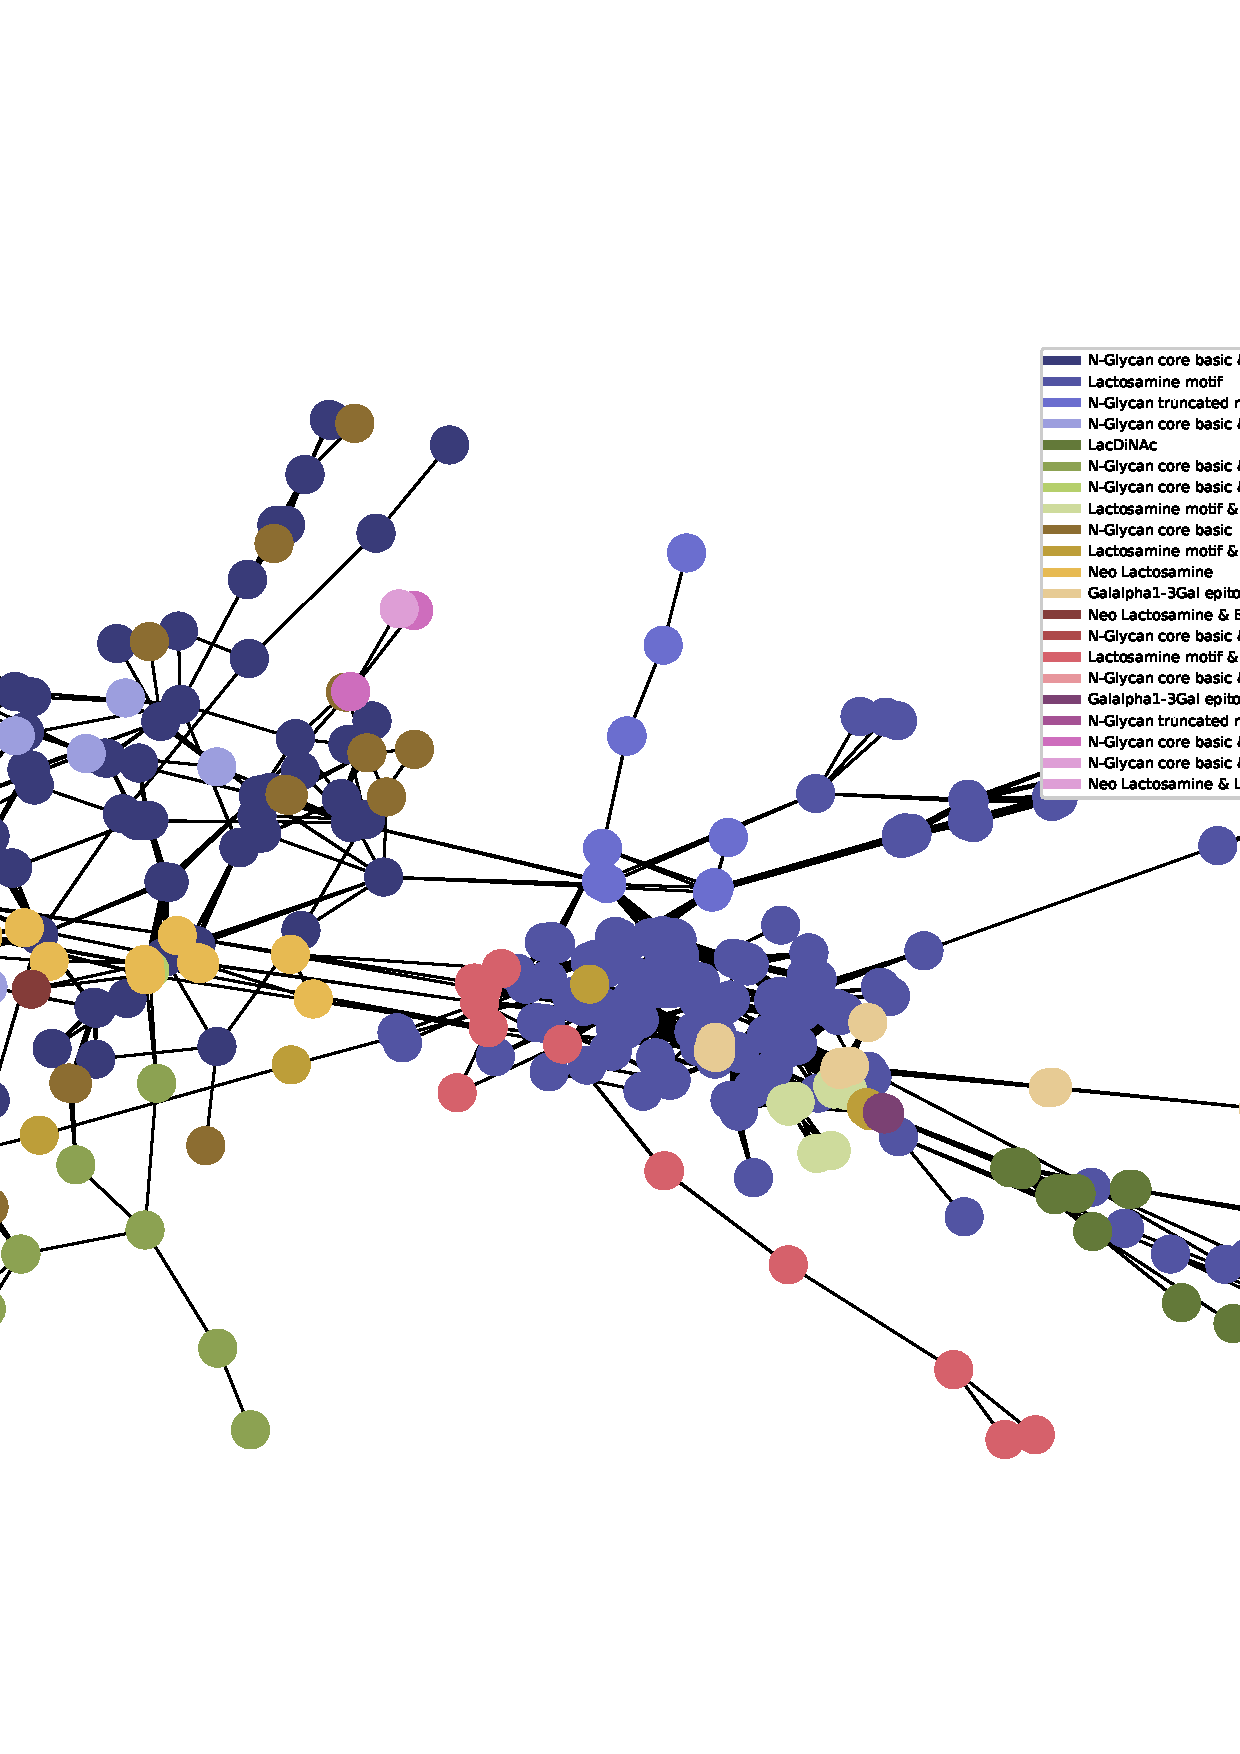
\includegraphics[scale=0.5]{threshold_87_conn_comp_1_method_set/threshold_87_conn_comp_1_method_set.pdf} 
\caption{Most connected component of a network of glycans, with similarity determined using the reaction set method.}
\label{fig:threshold_87_conn_comp_1_method_set}
\end{sidewaysfigure}
\clearpage

\begin{figure}[H]
\centering 
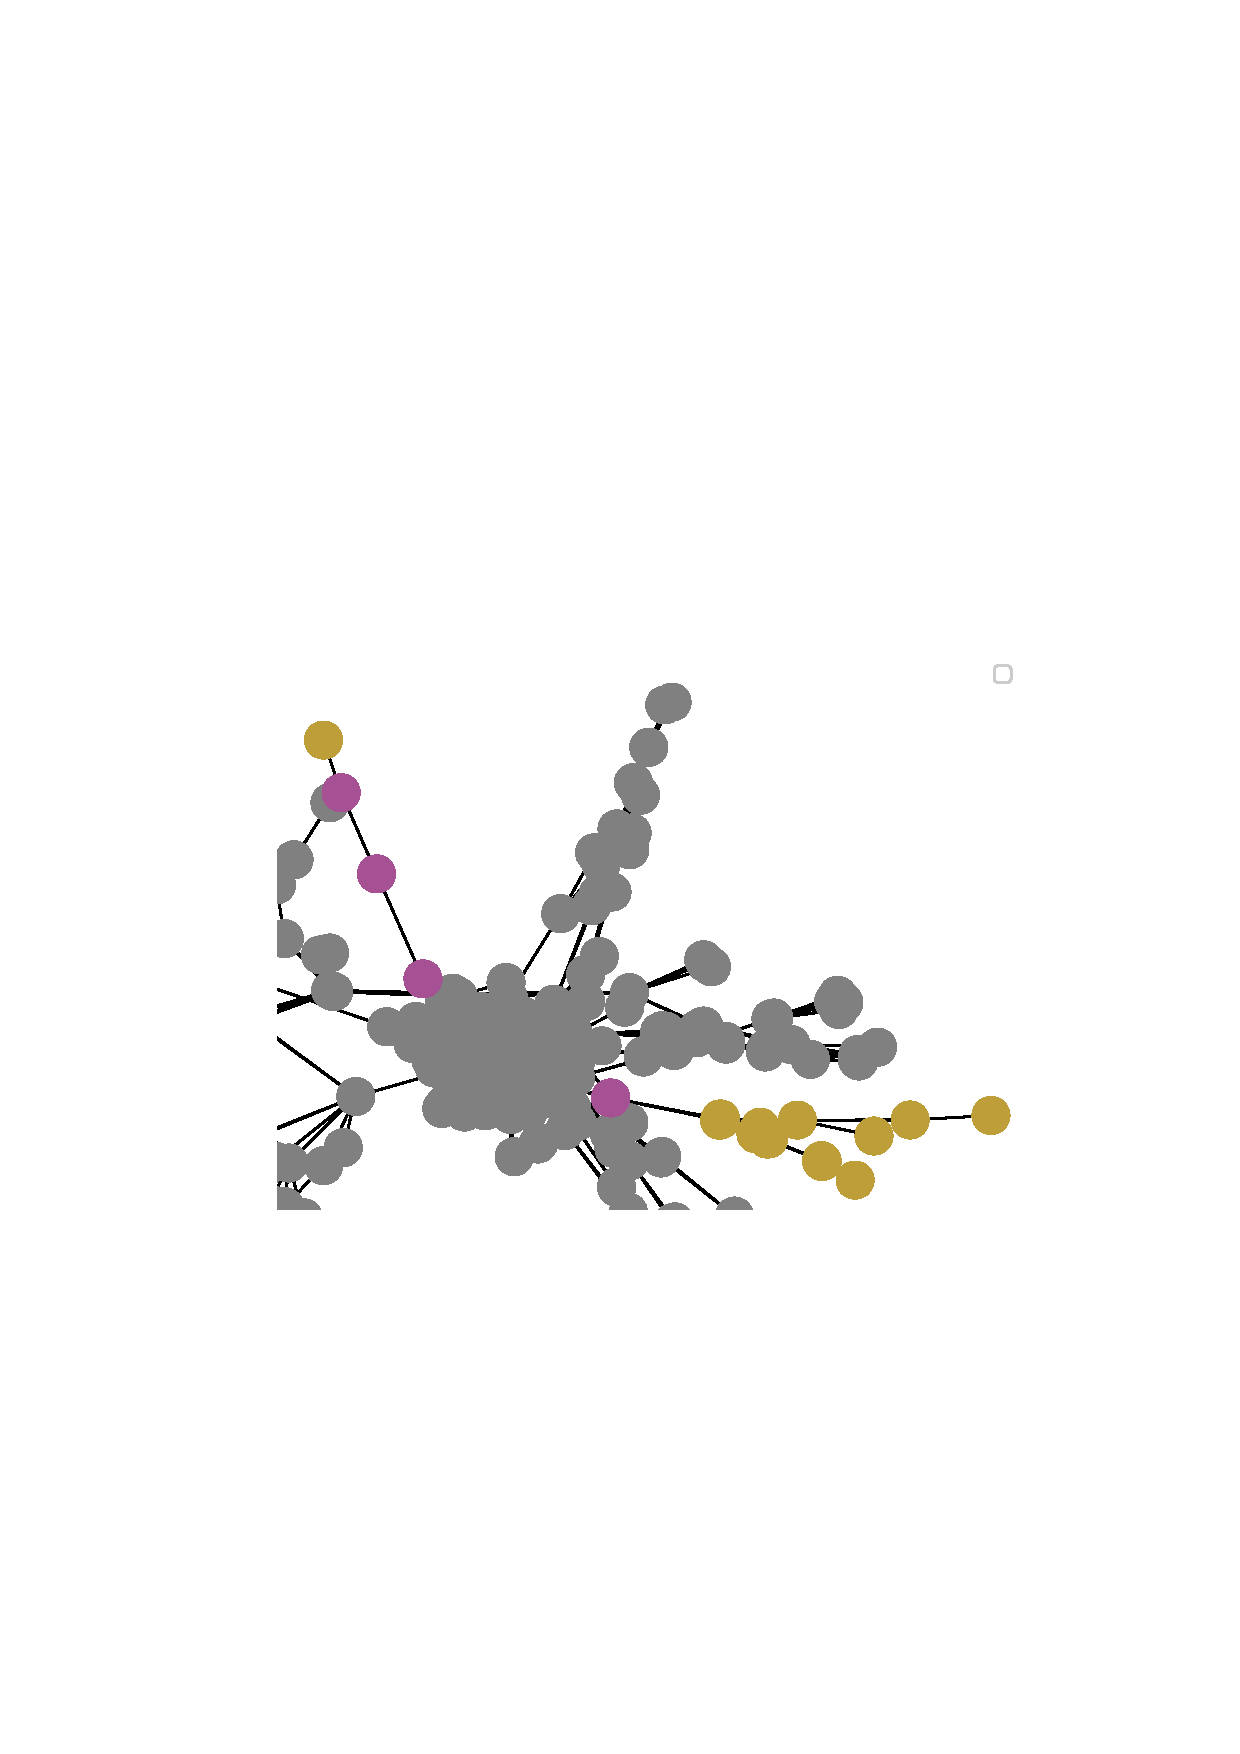
\includegraphics[scale=0.9]{motif_similarity_exploration/LacDiNAc_vs_Lactosamine_motif_LacDiNAc.pdf} 
\caption{Glycans containing the LacDiNAc motif (orange nodes) are connected solely to glycans containing the LacDiNAc and Lactosamine motifs (purple nodes).}
\label{fig:LacDiNAc_vs_Lactosamine motif,LacDiNAc}
\end{figure}

In Figure \ref{fig:LacDiNAc_vs_Lactosamine motif,LacDiNAc}, we highlight only two groups of glycans -- those containing the single motif LacDiNAc (coloured orange), and those containing two motifs -- LacDiNAc and the Lactosamine motif (coloured purple). All other glycans are coloured grey. In the same figure, we also display the glycan motifs. The two motif sets are similar to each other in two respects -- firstly, they both share exactly the same motif, LacDiNAc, and secondly, Lactosamine and LacDiNAc have in common a $\beta$ anomeric N-Acetyl-D-Glucosamine monosaccharide (the blue square). It is reasonable then to assume that glycans containing either of these motif sets would be structurally similar, and indeed the figure illustrates that the glycans in our network with just the LacDiNAc motif  (orange) are solely connected either to each other or to glycans containing the LacDiNAc and Lactosamine motifs.

Another example is shown in Figure \ref{fig:Galalpha1-3Gal_epitope_Lactosamine_motif_Blood_group_H_vs_Lactosamine_motif_Blood_group_H}, this time highlighting glycans containing the Galalpha1-3Gal epitope, Lactosamine, and Blood group H motifs (orange), and those containing Lactosamine, and Blood group H motifs (green). Direct connections exist between the two groups, as we would expect given that one group contains two out of the three motifs present in the other.

\begin{figure}[H]
\centering 
\includegraphics[scale=0.85]{motif_similarity_exploration/Galalpha1-3Gal_epitope__Lactosamine_motif__Blood_group_H_vs_Lactosamine_motif__Blood_group_H.pdf} 
\caption{Glycans containing the Galalpha1-3Gal epitope, Lactosamine, and Blood group H motifs (orange nodes) are connected to glycans containing the Lactosamine, and Blood group H motifs (green nodes).}
\label{fig:Galalpha1-3Gal_epitope_Lactosamine_motif_Blood_group_H_vs_Lactosamine_motif_Blood_group_H}
\end{figure}

Conversely, in each of Figures \ref{fig:N-Glycan_core_basic_vs_Lactosamine_motif} and \ref{fig:Neo_Lactosamine_vs_LacDiNAc}, we highlight two groups of glycans which do not share similar motifs. In these instances, there are no direct connections between the two glycan groups, implying significant structural differences, as we would expect given the differences in motifs. Network graphs created using the reactions list method, as opposed to the reactions set method, exhibit the same types of relationships and we omit them here.

\begin{figure}[H]
\centering 
\includegraphics[scale=0.9]{motif_similarity_exploration/N-Glycan_core_basic_vs_Lactosamine_motif.pdf} 
\caption{Glycans containing the N-Glycan core basic motif (green nodes) are not directly connected to glycans containing the Lactosamine motif (blue nodes).}
\label{fig:N-Glycan_core_basic_vs_Lactosamine_motif}
\end{figure}

\begin{figure}[H]
\centering 
\includegraphics[scale=0.9]{motif_similarity_exploration/Neo_Lactosamine_vs_LacDiNAc.pdf} 
\caption{Glycans containing the Neo Lactosamine motif (orange nodes) are not directly connected to glycans containing the LacDiNAc motif (violet nodes).}
\label{fig:Neo_Lactosamine_vs_LacDiNAc}
\end{figure}

\newpage
\subsection{Assortativity Coefficient}
\label{sec:assortativity_coefficient}

The assortativity coefficients calculated for the two alternative similarity measures are:\\

Reaction set method: {\bf 0.93}\\
\indent Reaction list method {\bf 0.97}\\

The higher value for the reaction list method suggests that there is a benefit to taking into account reaction quantities, rather than just presence, when measuring glycan similarity.

\subsection{UPGMA Hierarchical Clustering}
\label{sec:clustering_results}

Figure \ref{fig:full_tree_zoomed} shows a magnified section of the full tree (in cladogram form) produced using UPGMA hierarchical clustering, applied to the distance matrix obtained using the reaction list method. The 4111 terminal nodes, which represent individual glycans, are labelled with both the names of the motifs present in each glycan, and, in brackets, the glycan ID (as taken from the GlyTouCan database). The visualisation software dynamically adjusts the number of terminal nodes for which it displays labels in order to avoid clutter. We can see via the terminal labels and the branch colours that there are distinct clades of glycans which share the same motif sets, providing further evidence of the suitability of our method for determining glycan similarity. Furthermore, adjacent clades of different colours often have motifs in common, analogous to the connected nodes we observed in the glycan network.

\begin{sidewaysfigure}
\centering 
\includegraphics[scale=0.3]{trees/zoomed_full_tree_cladogram.png} 
\caption{Full depth UPGMA tree (zoomed in to subsection). Clades of equal colour indicate clusters of glycans sharing the same motif sets.}
\label{fig:full_tree_zoomed}
\end{sidewaysfigure}
\clearpage

\subsubsection{Motif Discovery}
A detailed inspection of the UPGMA tree reveals some features which, initially, seem to be at odds with the notion of shared motifs between similar glycans observed so far. For example, in Figure \ref{fig:full_tree_LacDiNAc}, a glycan with the sole motif LacDiNAc (highlighted in red) appears amongst a cluster of glycans containing only the `N-Glycan truncated motif first GlcpNAC cut off' motif. However, looking up the structure of this glycan in the GlyTouCan database\footnote{\url{https://glytoucan.org/Structures/Glycans/G35645QP}} reveals that this glycan does in fact contain the `N-Glycan truncated motif first GlcpNAC cut off' motif as well as LacDiNAc, it just has not been annotated as containing it. Figure \ref{fig:rogue_lacdinac_a} shows the full glycan structure, Figure \ref{fig:rogue_lacdinac_b} shows the LacDiNAc motif, with which the glycan has been correctly annotated, and Figure \ref{fig:rogue_lacdinac_c} shows the `N-Glycan truncated motif first GlcpNAC cut off' motif which the glycan has not been annotated as containing, but which is clearly seen in the full structure (Figure \ref{fig:rogue_lacdinac_a}). We cannot rule out though the possibility that there is some positional dependency associated with the `N-Glycan truncated motif first GlcpNAC cut off' motif which precludes it from being declared as a motif for this particular glycan.


\begin{sidewaysfigure}
\centering 
\includegraphics[scale=0.3]{trees/rogue_LacDiNAc_in_tree.png} 
\caption{A glycan (highlighted in red) which has a missing motif annotation in the GlyTouCan database has been correctly clustered with glycans sharing the same motif.}
\label{fig:full_tree_LacDiNAc}
\end{sidewaysfigure}
\clearpage

\begin{figure*}[ht!]
    \centering
    \begin{subfigure}[t]{1.0\textwidth}
        \centering
        \includegraphics[scale=0.6]{trees/rogue_LacDiNAc_structure.png}
        \caption{Actual structure of the glycan highlighted in red in Figure \ref{fig:full_tree_LacDiNAc}.}
        \label{fig:rogue_lacdinac_a}
    \end{subfigure}%
    \\
    \bigbreak
    ~ 
	\\
    \begin{subfigure}[t]{1.0\textwidth}
        \centering
        \includegraphics[scale=0.6]{trees/LacDiNAc_motif.png}
        \caption{Correctly annotated LacDiNAc motif.}
        \label{fig:rogue_lacdinac_b}
    \end{subfigure}
    \\
    \bigbreak
    ~ 
	\\
    \begin{subfigure}[t]{1.0\textwidth}
        \centering
        \includegraphics[scale=0.6]{trees/N-Glycan_truncated_motif__First_GlcpNAC_cut_off_motif.png}
        \caption{Missing motif annotation `N-Glycan truncated motif First GlcpNAC cut off'}
        \label{fig:rogue_lacdinac_c}
    \end{subfigure}
    \caption{The actual structure of the glycan highlighted in red in Figure \ref{fig:full_tree_LacDiNAc} and its present and missing motif annotations.}
\label{fig:rogue_lacdinac}
\end{figure*}


\newpage
\section{Discussion}
\label{sec:discussion}

The same-motif glycans displayed in both the connected communities of  our network graphs and the clades of the UPGMA tree, as well as the discovery of the missing motif annotation for a particular glycan, are highly encouraging outcomes. These were found using just 4111 glycans from an original set of 105050 in the GlyTouCan database. Increasing the number of glycans in our analysis would open up the possibility of yet more insights of a similar nature. One straightforward way to achieve this would be to simply employ more computing resources -- this study was carried out on a single moderately powerful desktop machine. Beyond that though, we currently reject a large number of glycans because of experimental uncertainty in their structure. It should be possible to modify our parsing technique to make use of some of the certain glycan reactions contained within gycans whose overall structure contains ambiguities, therefore increasing our overall coverage.

The results we present here are produced using a technique based upon characterisation of glycans in terms of the reactions necessary to construct them. Glycans exhibit a tree-like structure, which we do not take into account. Measuring distance between tree structures is inherently more complex than the technique we present here, and it would be instructive to make a comparison between this approach and one which accounts for the specific tree-like nature of glycan structure, such as glycan classification with tree kernels \citep{doi:10.1093/bioinformatics/btm090}.

In Section \ref{sec:assortativity_coefficient} we report and compare the network assortativity coefficients for the networks produced by our two alternative glycan similarity measurement techniques. To increase our confidence in these values we should also determine their statistical significance. The script \texttt{bootstrap\_assortativity.py} is included in the source code for this project, which uses the `bootstrap' \citep{efron1992bootstrap} method to determine the means and standard deviations of the coefficients. Computation time for this script is high though, and the results were not available at the time of publication.



\newpage
\section{Further Work}
\label{sec:further_work}

In Sections \ref{sec:glycan_databases} and \ref{sec:extracting_reactions} we describe querying the GlyTouCan database using SPARQL queries, and later parsing the WURCS format string in order to obtain a list of reactions for each glycan. In fact, the GlyTouCan RDF data already provides a breakdown of more fine-grained elements of the full WURCS string, which offers us the opportunity to increase the amount of glycan reactions in our dataset via the use of alternative SPARQL queries. Suggestions for exploratory SPARQL queries are given in Appendix \ref{sec:sparql_queries}.

The visualisations created from our glycan networks are a valuable tool for exploring glycan similarity. The obvious communities of glycans sharing the same motif sets gives us confidence that our technique for measuring glycan similarity from their reactions is valid, and the spatial positioning offers some qualitative, if not quantitative, assessment of glycan similarity both within and between those communities of same motif set glycans. We present some static images here, however the full value of the visualisations is only realised when viewed live and interactively on a computer. We use the Python Matplotlib \citep{Hunter:2007} package to display our networks, which allows the user to zoom in and move the image up/down/left/right. This also seems somewhat limited though, and a custom visualisation tool would enhance the value of the networks. For example, there is useful motif, structure, and similarity coefficient information which could be displayed when clicking or hovering over nodes and edges. Groups of glycans could be dynamically selected, either by mouse clicking or via a search mechanism, and compared against one another. Rendering the images in three rather than two dimensions would also be useful. Possible visualisation tools include Cytoscape \citep{shannon2003cytoscape} and Large Graph Layout \citep{adai2004lgl}.

A key factor in producing useful network visualisations is the choice of threshold value applied to the similarity matrix, in order to then reduce it down to a binary adjacency matrix. A value too high will result in only glycans with near identical structure forming connections, whilst too low will result in connections between unrelated glycans. This is not seen to be a major problem, as we are free to manipulate the networks as we please in order to maximise their utility. However it does leave open the question of where do we draw the line between similar and dissimilar glycans -- further work to define this boundary would be useful.

When performing hierarchical clustering (Section \ref{sec:clustering}, we used the UPGMA algorithm. Other algorithms could be employed here, and could potentially offer gains in terms of computation time. One example, the Bit-Pattern Biclustering (BiBit) Algorithm \citep{rodriguez2011biclustering}, claims good performance when applied to large datasets, such as gene expression data. 

The dataset we use here solely provides details of glycan structure, including motifs. A dataset of glycan samples by cell and tissue type exists \citep{cfg_dataset}, which provides an opportunity to (for example) make comparisons between glycan structures in disease state and non-disease state cells or tissues. We provide a Python script, \texttt{glycan\_scraper.py} for downloading the data from this website, however the data is in a different format (MSA) to that required by our software (WURCS). There are tools available \citep{Glycome_Analytics_Platform} which can convert from MSA to another format, `linearcode', and then to WURCS, however in our tests the conversion from linearcode to WURCS was not able to deal with data in which uncertainties in the glycan structure are expressed, and consequently further development of the conversion tools is required in order to proceed with this dataset.

In Table 1 of \citep{porter2009motif}, some rules governing glycan structure in relation to motifs are given. For example, the definition given for the N-Glycan hybrid motif is ``A glycan chain with a Mana1-3(Mana1-6)Manb1-4GlcNAcb1-4GlcNAcb base with GlcNAcb1-2 linked to only one of the two terminal mannose glycans (Mana1,3 or Mana1,6); the branch with the GlcNAcb1,2 can continue to grow with any glycan, but only mannose may be present on the other mannose''. An extension of the tools we present here could be used to validate these rules, for example by modelling glycans which break the rules and then searching for real examples of high similarity.

\newpage
\section{Conclusions}
\label{sec:conclusions}

Measuring similarity between glycans is challenging due to their complex tree-like structure and the high number of both constituent monosaccharides and the types of glycosidic links between them. We have demonstrated encouraging results based upon a novel technique of determining glycan similarity which avoids the need to carry out complex comparisons of tree structures, allowing us to explore similarities both within and between communities of glycans sharing the same or similar sets of motifs. Our technique enables the identification of previously unlabelled motifs in glycans, and we provide several suggestions for advancing this research further. Of particular interest is the possibility of using the cell and tissue-specific glycan dataset in order to broaden the scope of the research into identifying glycan structures associated with disease states.

We present network graph and cladogram images offering a qualitative validation of the technique, and would encourage the adaptation of the computer code provided such that our results might be visualised and explored further using more advanced imaging software.

Some relatively straightforward modifications to the method of querying the glycan database, and the use of more powerful computing resources, open up the possibility of vastly increasing the number of glycans analysed, and we provide the necessary computer script to determine the statistical significance of our quantitative results in order to further validate the technique.

\newpage
\bibliographystyle{agsm}
\bibliography{bibliography}


\newpage
\section*{Appendices}
\appendix
%\chapter{}
\section{Software Dependencies}
\label{sec:software_dependencies}
Table \ref{tab:software_dependencies} lists the packages necessary to run the python code used to produce the results described in this paper. The program code itself can be cloned into the current directory by typing the following command in a command window (assuming the Git\footnote{\url{https://git-scm.com/}} application is already installed):

\begin{verbatim}
git clone https://github.com/ImperialCollegeLondon/glycans.git
\end{verbatim}

\begin{table}[h]
\centering
%\resizebox{\columnwidth}{!}
\rowcolors{1}{}{lightblue}
\begin{tabular}{|c|c|} \hline
{\bf Package Name} & {\bf Version} \\ \hline
biopython   &               1.72 \\ \hline
fontconfig    &             2.12.6 \\ \hline
glypy       &               0.12.2 \\ \hline
html5lib   &                1.0.1 \\ \hline
httplib2   &                0.11.3 \\ \hline
matplotlib &                2.2.2 \\ \hline
networkx  &                 2.1 \\ \hline
numpy    &                  1.14.3 \\ \hline
numpy-base   &              1.14.5 \\ \hline
pandas  &                   0.23.2 \\ \hline
python   &                  3.6.6 \\ \hline
rdflib  &                   4.2.2 \\ \hline
scipy   &                   1.1.0 \\ \hline
seaborn  &                  0.8.1 \\ \hline
sparqlwrapper   &           1.8.0 \\ \hline
urllib3      &              1.23 \\ \hline
\end{tabular}
\caption{Python software packages necessary to run the program code associated with this project.}
\label{tab:software_dependencies}
\end{table}
\clearpage

%\chapter{}
\section{Glycan Databases and Structure Formats}
\label{sec:glycan_dbs_and_formats}
Table \ref{tab:glycan_databases} lists some glycan databases, the number of glycans they contain, and the glycan structure formats they provide.

\begin{table}[h]
\begin{minipage}{\textwidth}
\centering
%\resizebox{\columnwidth}{!}
\rowcolors{1}{}{lightblue}
\begin{tabular}{|c|c|p{7cm}|} \hline
{\bf Database Name} & {\bf No. glycans}  & {\bf Formats} \\ \hline
KEGG Glycan\footnote{\url{https://www.genome.jp/dbget-bin/www_bfind_sub?mode=bfind&max_hit=1000&locale=en&serv=gn&dbkey=glycan&keywords=*&page=1}} & 504 & KCF \\ \hline
GlyConnect\footnote{\url{https://glyconnect.expasy.org/browser/structures/2259}} & 3768 & IUPAC \\ \hline
UniCarbKB\footnote{\url{http://www.unicarbkb.org/}} & 3238 & note\footnote{Website not working at time of publication} \\ \hline
GlyTouCan\footnote{\url{https://glytoucan.org/}} & 105050 & WURCS, GlycoCT, IUPAC Condensed, IUPAC Extended \\ \hline
\end{tabular}
\caption{Glycan databases, and the structure formats they provide.}
\label{tab:glycan_databases}
\end{minipage}
\end{table}

\noindent Different glycan structure formats exist. The number of glycans in the GlyTouCan database for each format it supports are shown in Table \ref{tab:glycan_format_counts}.

\begin{table}[h]
\centering
\rowcolors{1}{}{lightblue}
\begin{tabular}{|c|c|c|} \hline
{\bf Format Name} & {\bf Number of Glycans} & {\bf Comments} \\ \hline
GlycoCT & 45438 & Verbose, no longer supported\\ \hline
IUPAC & 14517 & \\ \hline
IUPAC condensed & 73329 & \\ \hline
IUPAC extended & 73329 & \\ \hline
WURCS & 105050 & Most recently published \\ \hline
\end{tabular}
\caption{Glycan counts in the GlyTouCan database for different glycan structure formats.}
\label{tab:glycan_format_counts}
\end{table}

\singlespace
\noindent Additional glycan resources can be found at the following URLs:
\begin{itemize}
\item \path{https://biosciencedbc.jp/en/db-link/d09-dblink}
\item \path{http://www.functionalglycomics.org/static/consortium/links.shtml}
\item \path{https://biosciencedbc.jp/en/db-link/d09-dblink}
\end{itemize}
\doublespace
\clearpage

\section{SPARQL queries}
\label{sec:sparql_queries}
SPARQL queries may be run programmatically, or against the GlyTouCan database at the following `SPARQL Endpoint' (a web query interface):\\

\noindent \path{https://ts.glytoucan.org/sparql}\\

\noindent The following SPARQL query returns all Glycan IDs, WURCS format strings, and motif IDs. Results for glycans with multiple motifs will be spread across multiple lines:

\singlespace
\begin{verbatim}
  PREFIX glycan: <http://purl.jp/bio/12/glyco/glycan#>
  PREFIX glytoucan:  <http://www.glytoucan.org/glyco/owl/glytoucan#>

  SELECT DISTINCT ?Saccharide ?PrimaryId ?Sequence 
                  ?Motif ?MotifPrimaryId
  FROM <http://rdf.glytoucan.org/core>
  FROM <http://rdf.glytoucan.org/sequence/wurcs>
  FROM <http://rdf.glytoucan.org/motif>
  WHERE {
    ?Saccharide glytoucan:has_primary_id ?PrimaryId .
    ?Saccharide glycan:has_glycosequence ?GlycoSequence .
    ?GlycoSequence glycan:has_sequence ?Sequence .
    ?GlycoSequence glycan:in_carbohydrate_format 
      glycan:carbohydrate_format_wurcs.
    OPTIONAL { ?Saccharide glycan:has_motif ?Motif .
               ?Motif glytoucan:has_primary_id ?MotifPrimaryId } .
  }
  ORDER BY ?PrimaryId
\end{verbatim}
\doublespace

\newpage
\noindent This SPARQL query returns all Motif IDs and motif labels:

\singlespace
\begin{verbatim}
  PREFIX glycan: <http://purl.jp/bio/12/glyco/glycan#>
  PREFIX glytoucan:  <http://www.glytoucan.org/glyco/owl/glytoucan#>

  SELECT DISTINCT ?Motif ?MotifPrimaryId ?MotifLabel
  FROM <http://rdf.glytoucan.org/core>
  FROM <http://rdf.glytoucan.org/sequence/wurcs>
  FROM <http://rdf.glytoucan.org/motif>
  WHERE {
    ?Saccharide glycan:has_motif ?Motif .
    ?Motif glytoucan:has_primary_id ?MotifPrimaryId.
    ?Motif rdfs:label ?MotifLabel
  }
  ORDER BY ?MotifPrimaryId
  
\end{verbatim}
\doublespace

\noindent This SPARQL query is useful for exploring the glycan properties available in the GlyTouCan database, and returns a list of the distinct RDF properties within the full set of triples:

\singlespace
\begin{verbatim}
    SELECT DISTINCT ?p
    FROM <http://rdf.glytoucan.org/core>
    FROM <http://rdf.glytoucan.org/sequence/wurcs>
    FROM <http://rdf.glytoucan.org/motif>
    WHERE {
        ?s ?p ?o
    }
    
\end{verbatim}
\doublespace

\noindent A selection of results from the query above which could be useful for constructing new exploratory SPARQL queries are listed overleaf.\\

\newpage
\singlespace
{\scriptsize
\begin{verbatim}
http://purl.jp/bio/12/glyco/glycan#has_glycosequence
http://purl.jp/bio/12/glyco/glycan#has_resource_entry
http://purl.jp/bio/12/glyco/glycan#has_sequence
http://purl.jp/bio/12/glyco/glycan#in_carbohydrate_format
http://purl.jp/bio/12/glyco/glycan#in_glycan_database
http://purl.jp/bio/12/glyco/glycan#has_motif
http://www.glycoinfo.org/glyco/owl/wurcs#LIN_count
http://www.glycoinfo.org/glyco/owl/wurcs#RES_count
http://www.glycoinfo.org/glyco/owl/wurcs#has_GLIP
http://www.glycoinfo.org/glyco/owl/wurcs#has_GLIPS
http://www.glycoinfo.org/glyco/owl/wurcs#has_LIN
http://www.glycoinfo.org/glyco/owl/wurcs#has_MAP_position
http://www.glycoinfo.org/glyco/owl/wurcs#has_RES
http://www.glycoinfo.org/glyco/owl/wurcs#has_SC_position
http://www.glycoinfo.org/glyco/owl/wurcs#has_basetype
http://www.glycoinfo.org/glyco/owl/wurcs#has_direction
http://www.glycoinfo.org/glyco/owl/wurcs#has_monosaccharide
http://www.glycoinfo.org/glyco/owl/wurcs#has_rep_max
http://www.glycoinfo.org/glyco/owl/wurcs#has_rep_min
http://www.glycoinfo.org/glyco/owl/wurcs#has_root_RES
http://www.glycoinfo.org/glyco/owl/wurcs#has_uniqueRES
http://www.glycoinfo.org/glyco/owl/wurcs#is_fuzzy
http://www.glycoinfo.org/glyco/owl/wurcs#is_monosaccharide
http://www.glycoinfo.org/glyco/owl/wurcs#is_repeat
http://www.glycoinfo.org/glyco/owl/wurcs#is_uniqueRES
http://www.glycoinfo.org/glyco/owl/wurcs#uniqueRES_count
http://www.glycoinfo.org/glyco/owl/wurcs#has_modification_prob_lower
http://www.glycoinfo.org/glyco/owl/wurcs#has_modification_prob_upper
http://www.glycoinfo.org/glyco/owl/wurcs#has_MAP
http://www.glycoinfo.org/glyco/owl/wurcs#has_acceptor
http://www.glycoinfo.org/glyco/owl/wurcs#has_donor
http://www.glytoucan.org/glyco/owl/glytoucan#has_primary_id
http://www.glytoucan.org/glyco/owl/glytoucan#date_registered
http://www.glytoucan.org/glyco/owl/glytoucan#contributor
http://www.glycoinfo.org/glyco/owl/wurcs#has_root_GRES
http://www.glycoinfo.org/glyco/owl/wurcs#has_GRES
http://www.glycoinfo.org/glyco/owl/wurcs#is_acceptor_of
http://www.glycoinfo.org/glyco/owl/wurcs#has_acceptor_position
http://www.glycoinfo.org/glyco/owl/wurcs#has_donor_position
http://www.glycoinfo.org/glyco/owl/wurcs#is_donor_of
http://www.glycoinfo.org/glyco/owl/wurcs#count_RES
http://www.glycoinfo.org/glyco/owl/wurcs#count_uniqueRES
http://www.glycoinfo.org/glyco/owl/wurcs#count_LIN
http://www.glytoucan.org/glyco/owl/glytoucan#is_reducing_end
\end{verbatim}
}
\doublespace

\clearpage
\section{Illustrative WURCS Format String Example}
\label{sec:wurcs_example}

Figure \ref{fig:wurcs_example} (overleaf) illustrates the components of a WURCS format string, describing glycan structure. The corresponding brreakdown in terms of the biological reactions necessary for glycan synthesis is also shown.

\begin{sidewaysfigure}
\centering 
\includegraphics[scale=0.85]{images/wurcs_example.pdf} 
\caption{An example of glycan structure expressed in the WURCS format, with a corresponding breakdown in terms of child sugar, glycosidic link, and parent sugar. This breakdown is what we use to characterise glycans in terms of the biological reactions necessary for their synthesis.}
\label{fig:wurcs_example}
\end{sidewaysfigure}

\end{document}
